\documentclass[colorlinks]{thesis-kando}
\usepackage[T1]{fontenc}
\PassOptionsToPackage{defaults=hu-min}{magyar.ldf}
\usepackage[magyar]{babel}
\usepackage{pdfpages}
\usepackage{graphicx,amsmath,amssymb,amsthm,hulipsum,bussproofs}
\usepackage{listings,xcolor,rotating,booktabs,fancyvrb}
\usepackage{graphicx}
\usepackage{wrapfig}
\footnotestyle{rule=fourth}
\DeclareMathOperator{\tg}{tg}
\newtheorem{tetel}{Tétel}[chapter]
\newtheorem{lemma}[tetel]{Lemma}
\theoremstyle{definition}
\newtheorem{definicio}[tetel]{Definíció}
\newtheorem{feladat}[tetel]{Feladat}
\newtheorem{peldak}{Példák:}
\newtheorem{elonyok}{Előnyök}
\newtheorem{hatranyok}{Hátrányok}
\newtheorem{tortenet}{Története}
\newtheorem{miareact}{Mi az a React?}
\newtheorem{mitjel}{Mit is jelent ez?}
\newtheorem{mierhasz}{Miért hasznos ez nekünk?}
\newtheorem{apiveg}{API végpontok tesztelése}
\theoremstyle{remark}
\newtheorem{megjegyzes}[tetel]{Megjegyzés}
\newtheorem*{megoldas}{Megoldás}
\usepackage[normalem]{ulem}
\usepackage[linguistics]{forest}
\useunder{\uline}{\ul}{}
\usepackage{stackengine,scalerel}
\def\tang{\ThisStyle{\abovebaseline[0pt]{\scalebox{-1}{$\SavedStyle\perp$}}}}

\begin{document}
\institute{Informatika és távközlés ágazat}
\title{A szakdolgozat címe}
\author{Kiss Ákos\\Maklári Gábor\\Minka Dominik Elemér\\Szoftverfejlesztő és -tesztelő szak}
\supervisor{Kerényi Róbert Nándor\\oktató}
\city{Miskolc}
\date{2024}
\maketitle

\tableofcontents

\chapter*{Bevezetés}
\addcontentsline{toc}{chapter}{Bevezetés}

\textbf{MAMIK Bank}
\newline\newline
Miért választottuk ezt a témát?
\newline\newline
Közös megegyezés alapján, arra jutottunk, hogy a mai banki alkalmazások nem felelnek meg egy átlag ember elvárásainak.
Ezért úgy döntöttünk, hogy az összes banki applikációt kivesézzük az előnyeiről-hátrányairol, és az alkalmazások által
tanultakat megpróbáljuk szinkronba hozni hogy megalkossunk egy innovatív alkalmazást. Meg szeretnénk ismerkedni a bankok
minden napi tranzakcióival, működésével, felépítésével és nehézségeivel.
Mire nyújt megoldást?
\newline\newline
Szerettünk volna egy olyan banki tranzakciós applikációt létrehozni, aminek kikezdhetetlen a biztonsági rendszere,
biometrikus beléptetést nyújt az extra biztonság érdekében,felhasználóbarát(minden korosztálynak könnyű kezelést nyújt),
modern kezelőfelülettel rendelkezik a futurisztikus érzés átadásáért, egyszerüsíti a pénzgazdálkodást, reszponzív és bárhonnan(nemzetközileg is) hozzáférhető.
Mitől életszerű?
\newline\newline
Ez a banki alkalmazás életszerű, mert a felhasználók mindennapi pénzügyi szükségleteit szolgálja ki, legyen szó tranzakciókról,
fizetésekről, megtakarításról vagy biztonságos pénzkezelésről. Az emberek gyors, kényelmes és biztonságos megoldásokat keresnek a pénzügyeik kezelésére,
és egy banki alkalmazás pontosan ezt nyújtja.
\cite{Fazekas}
\chapter{Technológiák}

\section{Relációs adatbáziskezelő}

\subsection{Felépítés}
A relációs adatbázisok olyan rendszerek, amelyek adatokat tárolnak és kezelnek, és ezeket táblák formájában szervezik. Gondolj rájuk úgy, mint egy jól rendezett könyvtárra, ahol minden könyv (adat) egy adott kategóriában (táblában) van elhelyezve.
\subsection{Főbb jellemzők}

\begin{enumerate}
    \item Táblák: Az adatokat táblákba szervezzük, ahol minden tábla sorokból (rekordok) és oszlopokból (mezők) áll. Például, ha van egy „Könyvek” tábla, az oszlopok lehetnek: „Cím”, „Szerző”, „Kiadási év”.
    \item Kapcsolatok: A relációs adatbázisok lehetővé teszik a táblák közötti kapcsolatokat. Például egy „Könyvek” tábla és egy „Szerzők” tábla között létrejöhet egy kapcsolat, amely megmutatja, hogy melyik könyv ki által lett írva.
    \item Kérdezés: Az adatok lekérdezésére általában SQL-t (Structured Query Language) használnak. Ez egy speciális nyelv, amivel adatokat tudsz lekérdezni, hozzáadni, módosítani vagy törölni.
    \item Adatbiztonság: A relációs adatbázisok sokféle biztonsági megoldást kínálnak, például jogosultságokat, amelyek meghatározzák, ki férhet hozzá az adatokhoz.
\end{enumerate}
\begin{peldak}
    \begin{itemize}
        \item \mbox{} \\ Webáruházak: A termékek, vásárlók és rendelési adatok nyilvántartására.
        \item Iskolák: A diákok, tanárok és tantárgyak adatainak kezelésére.
    \end{itemize}
\end{peldak}

\section{PHP-MyAdmin - MySQL - MariaDB}

\subsection{PHPMyAdmin}
\begin{megjegyzes}
    A PHPMyAdmin egy webalapú alkalmazás, amely lehetővé teszi a MySQL és MariaDB adatbázisok kezelését. PHP-ban íródott, és a felhasználók grafikus felületen keresztül érhetik el az adatbázisokat.
\end{megjegyzes}

\begin{elonyok}

\begin{itemize}

    \item \mbox{} \\Felhasználóbarát: Könnyen használható grafikus felületet biztosít, amely segíti a felhasználókat az adatbázisok kezelésében.
    \item Funkciók: Támogatja a legtöbb MySQL/MariaDB funkciót, beleértve az adatbázisok létrehozását, módosítását, táblák kezelését, SQL lekérdezések futtatását stb.
    \item Platformfüggetlen: Mivel webalapú, bármilyen eszközről elérhető, amely rendelkezik böngészővel.

\end{itemize}
\end{elonyok}

\begin{hatranyok}
 
\begin{itemize}
    \item \mbox{} \\Teljesítmény: Nagy adatbázisok esetén lassabb lehet, mint a parancssori megoldások.
    \item Biztonsági kockázatok: Mivel webes alkalmazás, ha nem megfelelően van konfigurálva, biztonsági kockázatokat jelenthet (pl. SQL injection).
    \item Függőség: PHP és a webkiszolgáló (pl. Apache, Nginx) konfigurálása szükséges.
\end{itemize}
\end{hatranyok}
\subsection{MySQL}

\begin{megjegyzes}
    A MySQL egy népszerű, nyílt forráskódú relációs adatbázis-kezelő rendszer. A webfejlesztésben és más alkalmazásokban széles körben használják.
\end{megjegyzes}

\begin{elonyok}
    \begin{itemize}
        \item \mbox{} \\Stabilitás: Széles körben használt és megbízható, sok nagyvállalat is használja.
        \item Teljesítmény: Optimális teljesítményt nyújt, különösen nagy adatmennyiségek esetén.
        \item Széles körű támogatás: Nagy közösségi támogatás és dokumentáció, sokféle eszköz és könyvtár támogatja.
    \end{itemize}
    \end{elonyok}
    \mbox \\
    \begin{hatranyok}
    \begin{itemize}
        \item \mbox{} \\Licencdíjak: A MySQL Enterprise verziója díjköteles, míg a közösségi verzió korlátozottabb funkciókkal rendelkezik.
        \item Zárt forráskód: A MySQL egyes részei zárt forráskódúak, ami korlátozhatja a testreszabhatóságot.
    \end{itemize}
    \end{hatranyok}

\subsection{MariaDB}

\begin{megjegyzes}
    A MariaDB a MySQL forkja, amelyet az eredeti MySQL fejlesztői hoztak létre, miután a MySQL-t megvásárolta az Oracle. Célja, hogy a MySQL-hez hasonló, de nyílt forráskódú alternatívát kínáljon.
\end{megjegyzes}

\begin{elonyok}
    \begin{itemize}
        \item \mbox{} \\Teljesítmény: Számos optimalizálás van benne, ami javítja a teljesítményt, például a párhuzamos feldolgozás.
        \item Nyílt forráskód: Teljes mértékben nyílt forráskódú, így a felhasználók szabadon módosíthatják és terjeszthetik.
        \item Kompatibilitás: Nagy mértékben kompatibilis a MySQL-lel, így könnyen át lehet térni róla.
    \end{itemize}
    \end{elonyok}
    
    \begin{hatranyok}
    \begin{itemize}
        \item\mbox{} \\ Fiatalabb közösség: Bár a közössége növekszik, még nem olyan nagy és elterjedt, mint a MySQL-é.
        \item Egyes funkciók hiánya: Néhány MySQL funkció nem érhető el a MariaDB-ban, bár ez folyamatosan változik.
    \end{itemize}
    \end{hatranyok}

	
\includegraphics[width=15cm]{figures/relacios.jpg}


 \section{React Native}

 
\includegraphics[width=10cm]{figures/react.png}
\subsection{A React}
\begin{tortenet}
    \item \mbox \\-A React.js-t eredetileg a Facebook fejlesztette, ebből adódóan a Facebook is azt használja, valamint az Instagram. 2013-ban jelent meg.
\end{tortenet}
\begin{miareact}
    \item \mbox \\-A React egy deklaratív, effektív, és rugalmas JavaScript könyvtár, felhasználói felületek készítéséhez. Lehetővé teszi komplex felhasználói felületek összeállítását izolált kódrészletekből, amiket “komponenseknek” hívunk.
\end{miareact}
\begin{mitjel}
   
        
  
    \item Egy JavaScript könyvtár, amelyet
    felhasználói felületek, különösen
    egyoldalas alkalmazások "SPA"
    készítésére használnak.
    \item  komponensalapú: az alkalmazások
    kisebb, újrafelhasználható
    komponensekből állnak.
    \item hatékonyan kezeli a DOM-ot a "virtual
    DOM" segítségével.
    \item Deklaratív megközelítés, ahol a
    komponensek állapotváltozásai
    automatikusan frissítik a felhasználói
    felületet.
    \item Virtual DOM használata gyorsabb
    frissítéseket eredményez a
    felhasználói felületen.
    \item Nagyobb, összetett alkalmazások,
    amelyek sok felhasználói interakciót
    igényelnek.


\end{mitjel}
\newpage
\begin{mierhasz}
    \item -Felmerülhet bennünk a kérdés, hogy milyen esetekben érdemes használni ezeket a keretrendszereket, könyvtárakat? 
    \item A mai modern frontend keretrendszerek előnyei többek közt, hogy
   \begin{itemize}
  
  
    \item (pont)Könnyen használhatók
   \item (pont)Komponensekből állnak, melyeket újra hasznosíthatunk
    \item(pont)Strukturált, áttekinthető kódot biztosítanak számunkra
    \item(pont)Lehetőség nyílhat velük nem csupán "single-page" applikációk írására, így az "üzleti logika" jobban elkülöníthető
   \item (pont)Különféle állapotok jobban leírhatók vele
    \item(pont)Időt spórolnak meg számunkra
\end{itemize}
\end{mierhasz}
\subsection{React DOM és Virtual DOM}
\begin{itemize}
    \item React fő jellemzője a Virtual DOM használata, amely egy
    memóriában található DOM-reprezentáció.
    \item Amikor a React-ben valami változik, először ezt a Virtual
    DOM-ot frissíti.
    \item A Virtual DOM-ot aztán összehasonlítja a tényleges
    DOM-mal (diff algoritmus), és csak azokat a részeket frissíti
    a valódi DOM-ban, amelyek ténylegesen megváltoztak.
\end{itemize}
\subsection{Renderelési folyamat}
\begin{itemize}
    \item A komponens először a kezdeti állapottal (Helló, világ!)
    renderel.
    \item A felhasználó megnyomja a gombot, ami kiváltja a setMessage
    funkciót, amely frissíti az állapotot.
    \item A React látja, hogy az állapot változott, ezért újra rendereli a
    komponenst az új értékkel "Üzenet frissítve!".
    \item A DOM csak az új üzenetet frissíti, minden más változatlan
    marad.
    \item Az előbbi példa bemutatja a React alapvető renderelési
    logikáját, és azt, hogyan frissíti hatékonyan a felhasználói
    felületet az állapotváltozások alapján.

\end{itemize}
\subsection{React renderelés menete}
\begin{itemize}
    \item A React renderelési folyamata az, ami a komponensekből felépített
    virtuális DOM-ot összehasonlítja a valós DOM-mal, és hatékonyan frissíti
    azt, csak ott, ahol változások történtek. A React komponensek
    alapértelmezés szerint mindig újra renderelnek, amikor az állapotuk
    "state" vagy a kapott props-ok változnak.
    \item Főbb pontok:

    Renderelés: A komponensek JSX szintaxissal írnak HTML-szerű
    struktúrát, amit a React render() vagy funkcionális komponensek esetén
    maga a komponens visszatérési értéke kezel.
    \item Virtual DOM: A React a változtatásokat először egy memória alapú
    reprezentáción (virtual DOM) alkalmazza, majd csak azokat a részeket
    frissíti a tényleges DOM-ban, amelyek ténylegesen változtak.
    \item Újrarenderelés: A komponensek újra renderelődnek, ha az állapot (state)
    vagy a props változik, de a React hatékony diff algoritmussal kezeli a
    DOM frissítését.
    
\chapter{Projekt bemutatása}
A MAMIK Bank egy modern online banki platform, amely felhasználóbarát szolgáltatásokat kínál ügyfelei számára. Az oldal célja a pénzügyi biztonság és a könnyű pénzkezelés biztosítása.

\newpage
\section{Adatbázis bemutatása}
Ez az adatbázis egy banki rendszert modellez, amely különböző entitásokat kezel, mint például ügyfelek, számlák, tranzakciók, hitelkártyák és felhasználók.
\begin{figure}[h]
    \centering
    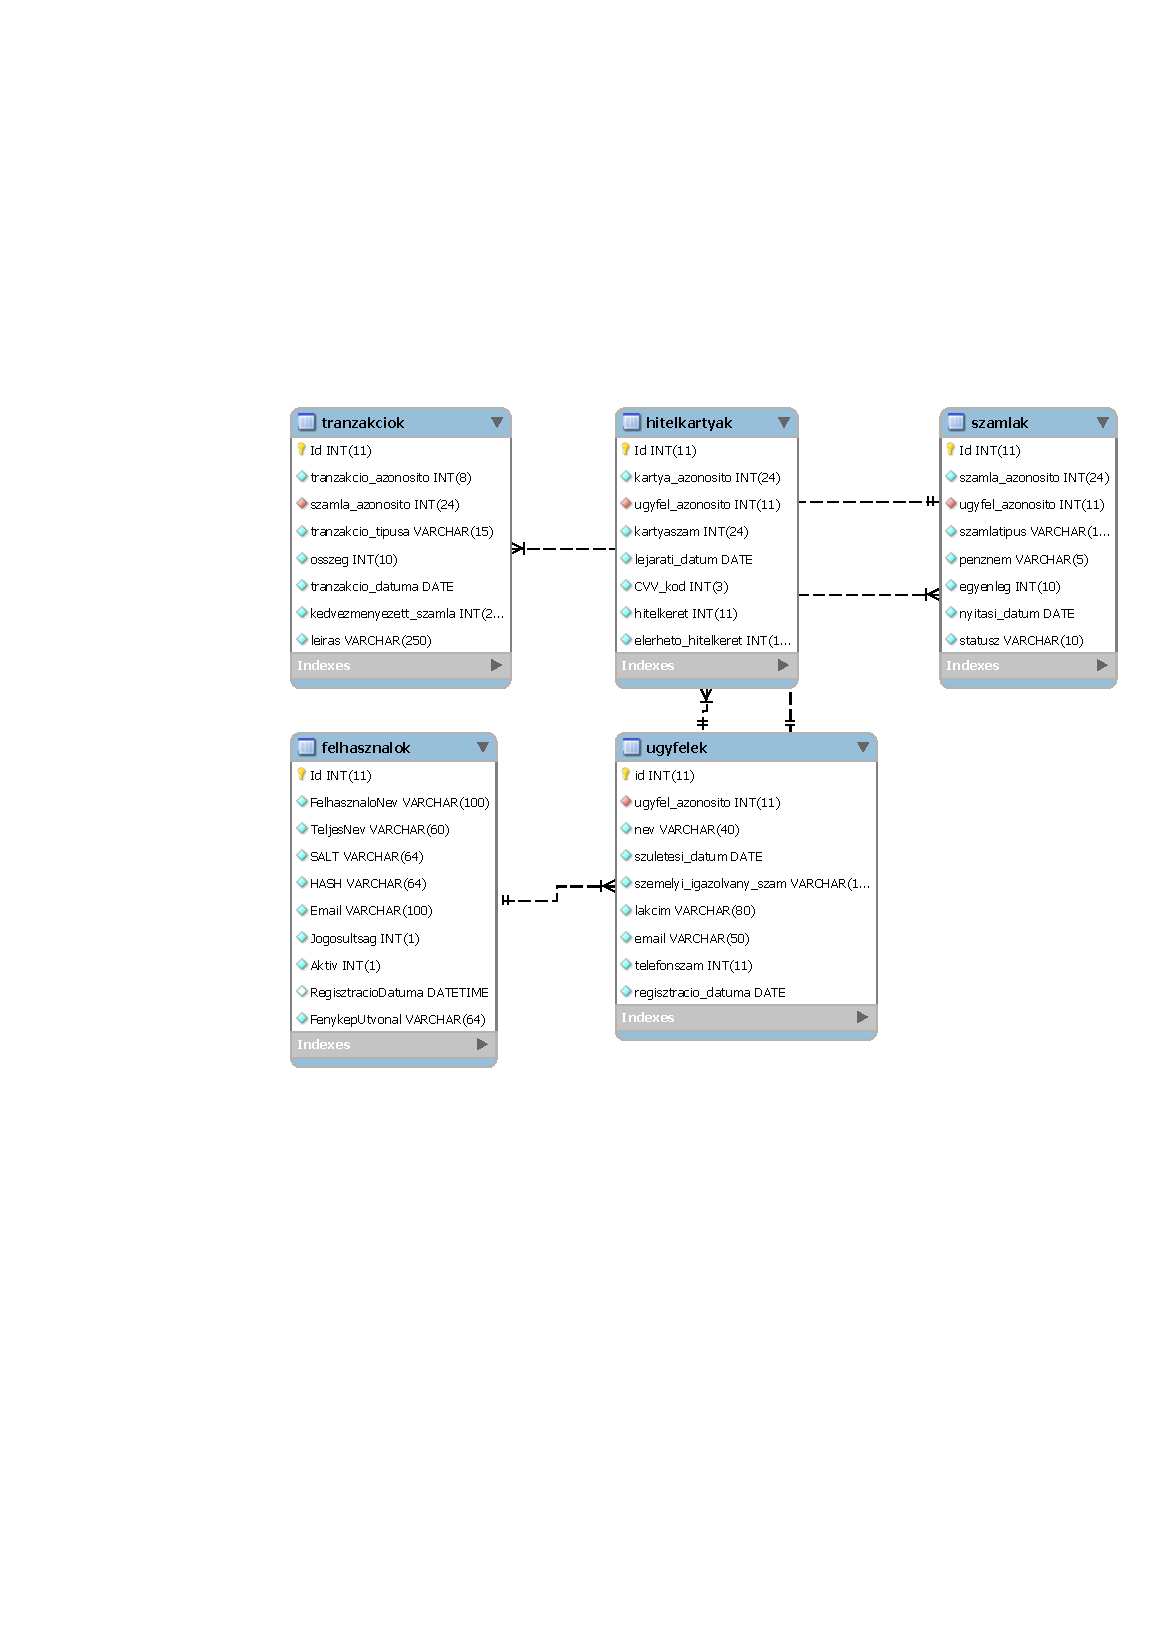
\includegraphics[width=10cm]{figures/adatb.pdf}
\end{figure}


\subsection{Tranzakciók}
\begin{itemize}
    \item \textbf{Id}: Egyedi azonosító
    \item \textbf{tranzakcio\_azonosito}: Tranzakció azonosító
    \item \textbf{szamla\_azonosito}: Kapcsolat a számlákkal
    \item \textbf{tranzakcio\_tipusa}: A tranzakció típusa (pl. befizetés, kifizetés)
    \item \textbf{osszeg}: Tranzakció összege
    \item \textbf{tranzakcio\_datum}: Tranzakció időpontja
    \item \textbf{kedvezmenyezett\_szamla}: Kedvezményezett számla azonosítója
    \item \textbf{leiras}: Tranzakció részletei
\end{itemize}

\subsection{Hitelkártyák}
\begin{itemize}
    \item \textbf{Id}: Egyedi azonosító
    \item \textbf{kartya\_azonosito}: Kártya azonosító
    \item \textbf{ugyfel\_azonosito}: Kapcsolat az ügyfelekkel
    \item \textbf{kartyaszam}: Hitelkártya száma
    \item \textbf{lejarati\_datum}: Lejárati dátum
    \item \textbf{CVV\_kod}: Biztonsági kód
    \item \textbf{hitelkeret}: Hitelkeret összege
    \item \textbf{elerheto\_hitelkeret}: Elérhető hitelkeret
\end{itemize}

\subsection{Számlák}
\begin{itemize}
    \item \textbf{Id}: Egyedi azonosító
    \item \textbf{szamla\_azonosito}: Számla azonosító
    \item \textbf{ugyfel\_azonosito}: Kapcsolat az ügyfelekkel
    \item \textbf{szamlatipus}: Számlatípus (pl. folyószámla, megtakarítási számla)
    \item \textbf{penznem}: Pénznem (pl. HUF, EUR)
    \item \textbf{egyenleg}: Számla egyenlege
    \item \textbf{nyitasi\_datum}: Nyitási dátum
    \item \textbf{statusz}: Számla állapota (pl. aktív, lezárt)
\end{itemize}

\subsection{Ügyfelek}
\begin{itemize}
    \item \textbf{Id}: Egyedi azonosító
    \item \textbf{ugyfel\_azonosito}: Ügyfél azonosító
    \item \textbf{nev}: Név
    \item \textbf{szuletesi\_datum}: Születési dátum
    \item \textbf{szemelyi\_igazolvany\_szam}: Személyi igazolvány szám
    \item \textbf{lakcim}: Lakcím
    \item \textbf{email}: Email cím
    \item \textbf{telefonszam}: Telefonszám
    \item \textbf{regisztracio\_datum}: Regisztráció dátuma
\end{itemize}

\subsection{Felhasználók}
\begin{itemize}
    \item \textbf{Id}: Egyedi azonosító
    \item \textbf{FelhasznaloNev}: Felhasználónév
    \item \textbf{TeljesNev}: Teljes név
    \item \textbf{SALT}: Titkosítás
    \item \textbf{HASH}: Jelszó hash
    \item \textbf{Email}: Email cím
    \item \textbf{Jogosultsag}: Jogosultsági szint
    \item \textbf{Aktiv}: Aktivitási állapot
    \item \textbf{RegisztracioDatuma}: Regisztráció dátuma
    \item \textbf{FenykepUtvonal}: Profilkép útvonala
\end{itemize}

\subsection{Kapcsolatok az Adatbázisban}
\begin{itemize}
    \item Az \textbf{ügyfelek} kapcsolódnak a \textbf{számlákhoz} és \textbf{hitelkártyákhoz}.
    \item A \textbf{számlák} kapcsolódnak a \textbf{tranzakciókhoz}.
    \item A \textbf{felhasználók} a rendszer adminisztrátori oldalához kapcsolódnak.
\end{itemize}
\newpage
\section{Backend bemutatása}
\begin{itemize}
    \item A MAMIK Bank backend egy ASP.NET Core alapú, MySQL adatbázist használó rendszer, amely biztonságosan kezeli az ügyféladatokat és tranzakciókat. A RESTful API biztosítja a gyors kommunikációt a frontend és backend között, míg a JWT token alapú hitelesítés és a szerepkör-alapú jogosultságkezelés védi az adatokat. A rendszer HTTPS és TLS titkosítással, bcrypt jelszóhasheléssel és SQL injection elleni védelemmel garantálja a biztonságot. Az indexelt adatbázis, caching és terheléselosztás növeli a teljesítményt és skálázhatóságot. Külső API-integrációkat támogat, lehetőséget adva további pénzügyi szolgáltatások beépítésére.
\end{itemize}
\subsection{Login és Logout}
\begin{itemize}
    \item \textbf{Bejelentkezés}: Az ügyfél fiókjába való belépés.
    \item \textbf{Kijelentkezés}: Az ügyfél biztonságos kilépése a rendszerből.
    \\
    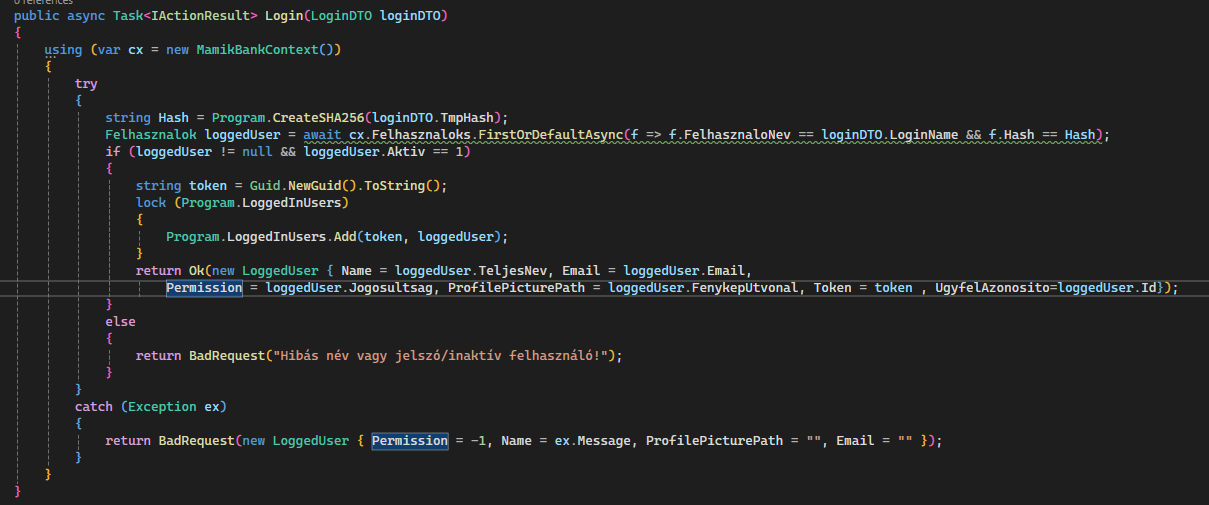
\includegraphics[width=10cm]{figures/bejel_backend.png}
\end{itemize}

\subsection{Regisztráció}
\begin{itemize}
    \item \textbf{Új ügyfél regisztrációja}: Új felhasználók hozzáadása a rendszerhez.
    \\
    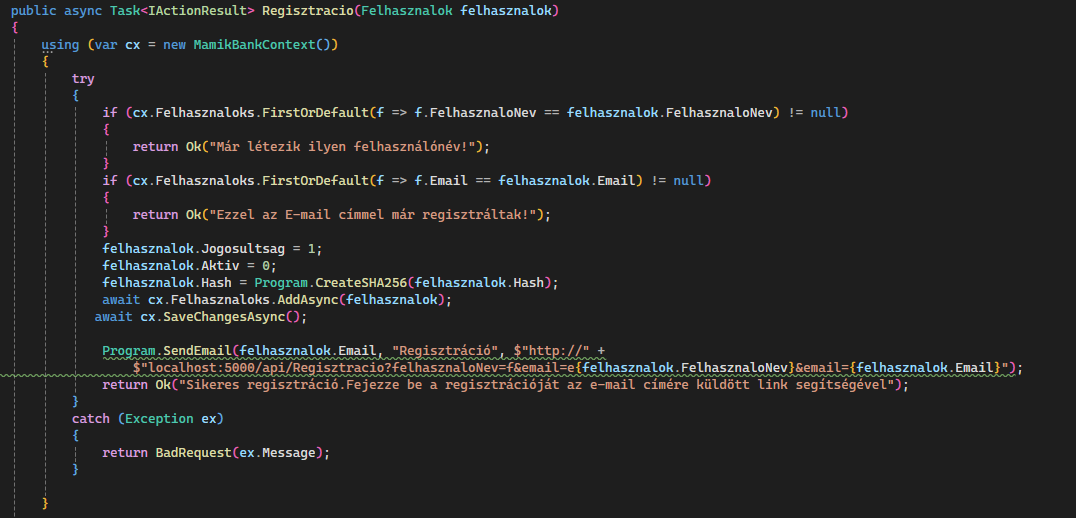
\includegraphics[width=10cm]{figures/reg_backend.png}

\end{itemize}

\subsection{Számlák}
\begin{itemize}
    \item \textbf{Számla lekérdezése}: Meglévő bankszámla adatainak lekérése.
    \\
    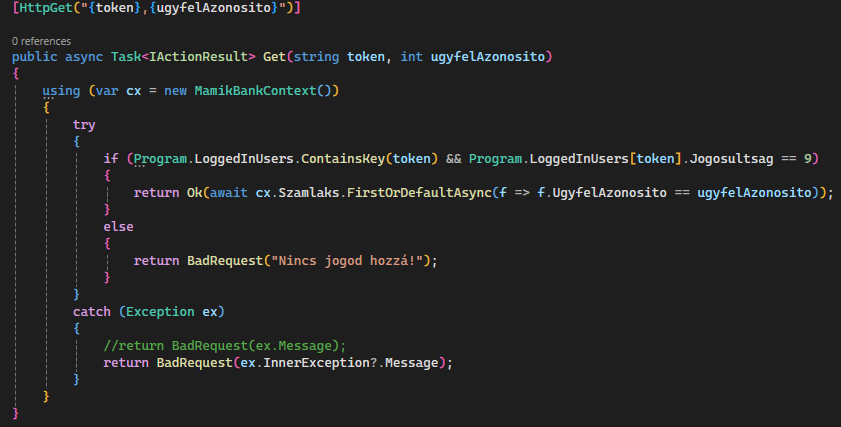
\includegraphics[width=8cm]{figures/szamlalekerdezes.png}
    \newpage
    \item \textbf{Számla létrehozása}: Új bankszámla megnyitása.
    \\
    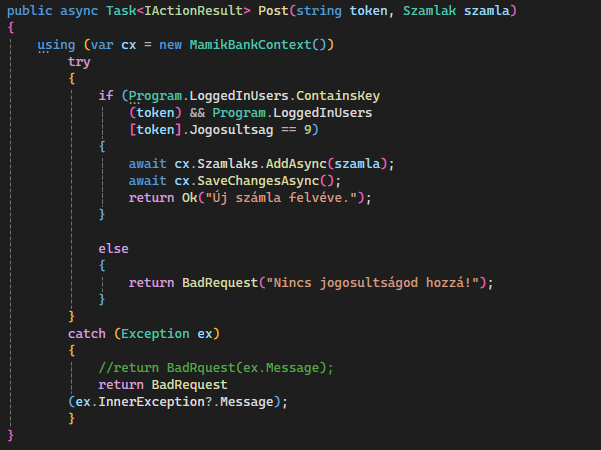
\includegraphics[width=8cm]{figures/szamlaletrehozas.png}
    \item \textbf{Számla módosítása}: Meglévő számlaadatok frissítése.
    \\
    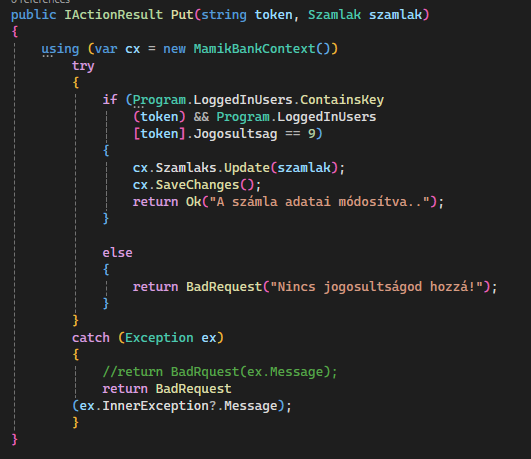
\includegraphics[width=8cm]{figures/szamlamodositas.png}
    \item \textbf{Számla törlése}: Meglévő számla törlése az adatbázisból.
    \\
    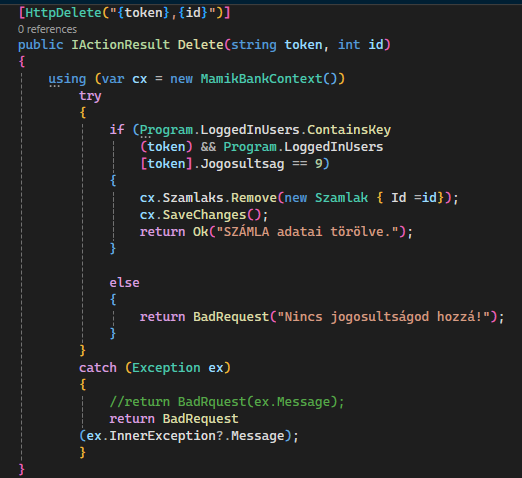
\includegraphics[width=8cm]{figures/szamlatorles.png}
\end{itemize}

\subsection{Tranzakciók}
\begin{itemize}
    \item \textbf{Tranzakciók lekérdezése}: Egy adott számlához kapcsolódó tranzakciók megtekintése.
    \\
    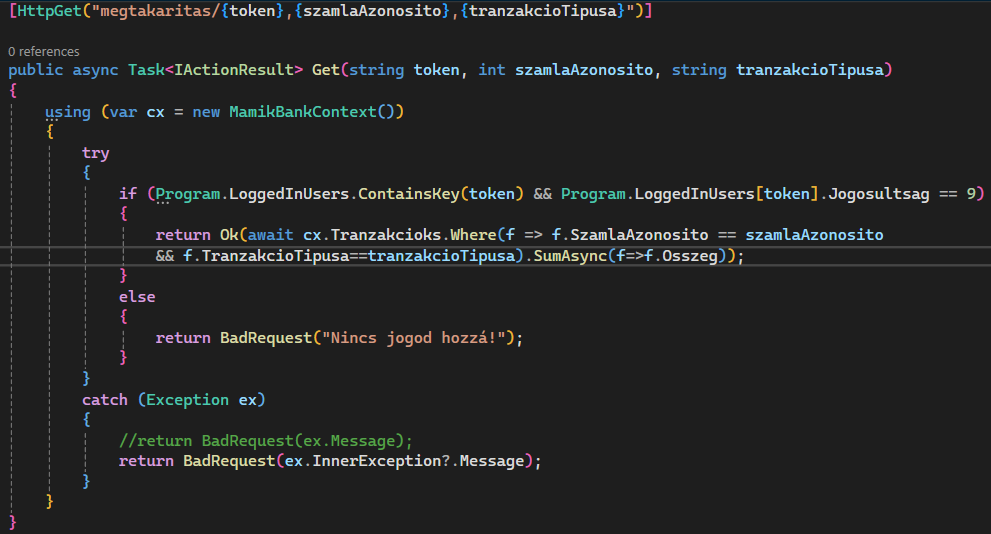
\includegraphics[width=10cm]{figures/tranzlekerdezes.png}
    \item \textbf{Új tranzakció létrehozása}: Új pénzügyi tranzakció indítása.
    \\
    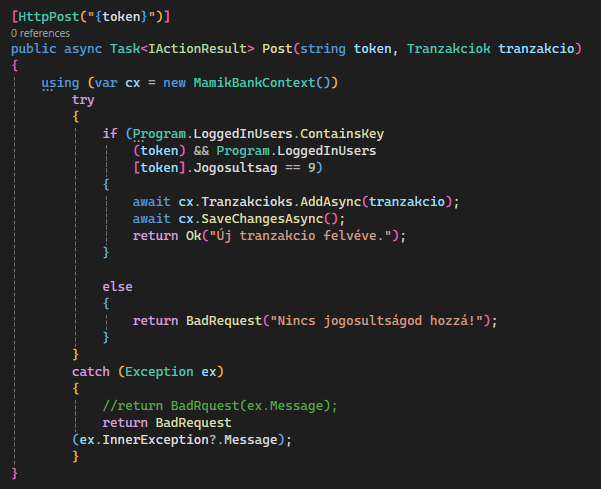
\includegraphics[width=8cm]{figures/tranzletrehozas.png}
    \item \textbf{Tranzakció módosítása}: Egy meglévő tranzakció frissítése.
    \\
    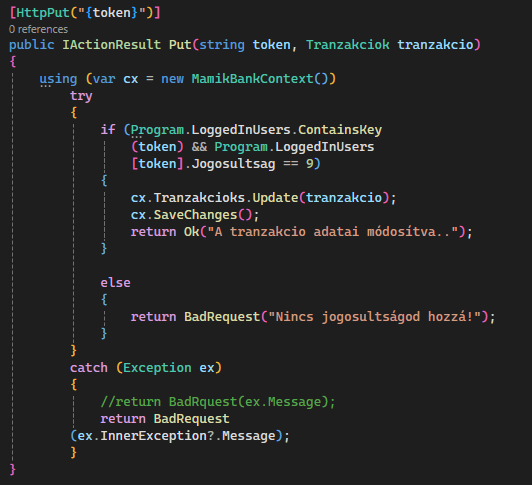
\includegraphics[width=8cm]{figures/tranzmodositas.png}
    \newpage
    \item \textbf{Tranzakció törlése}: Egy adott tranzakció törlése a rendszerből.
    \\
    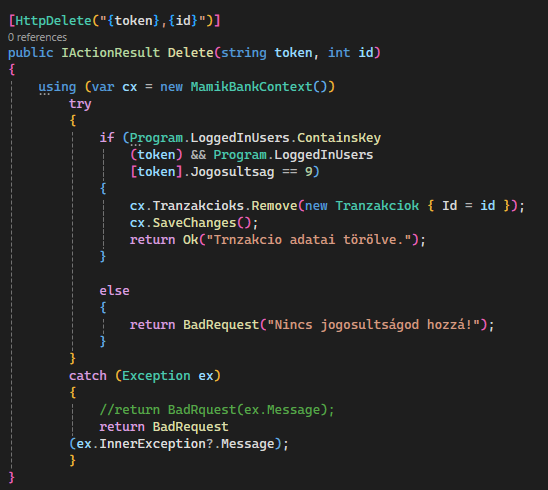
\includegraphics[width=8cm]{figures/tranztorles.png}
\end{itemize}

\subsection{Ügyfelek}
\begin{itemize}
    \item \textbf{Ügyféladatok lekérdezése}: Egy adott ügyfél adatainak megtekintése.
    \\
    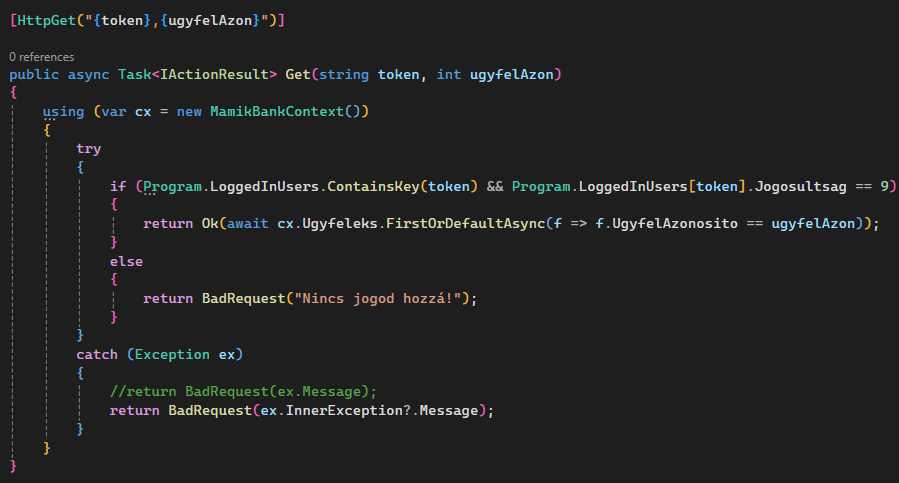
\includegraphics[width=8cm]{figures/ugyfellkerdezes.png}
    \item \textbf{Új ügyfél létrehozása}: Új ügyfél hozzáadása a rendszerhez.
    \\
    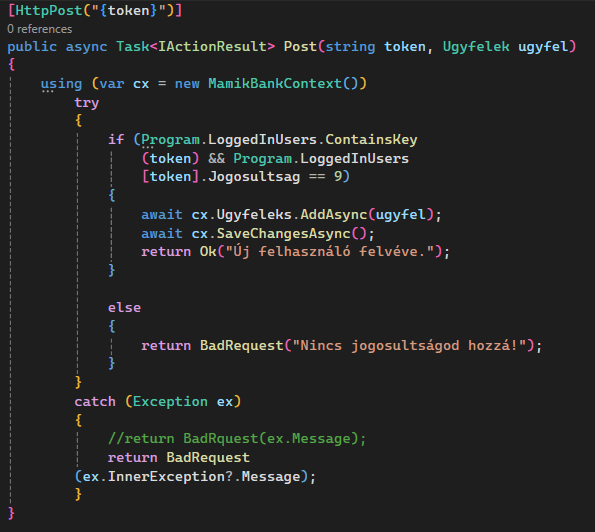
\includegraphics[width=8cm]{figures/ugyfelletrehozas.png}
    \newpage
    \item \textbf{Ügyféladatok frissítése}: Meglévő ügyféladatok módosítása.
    \\
    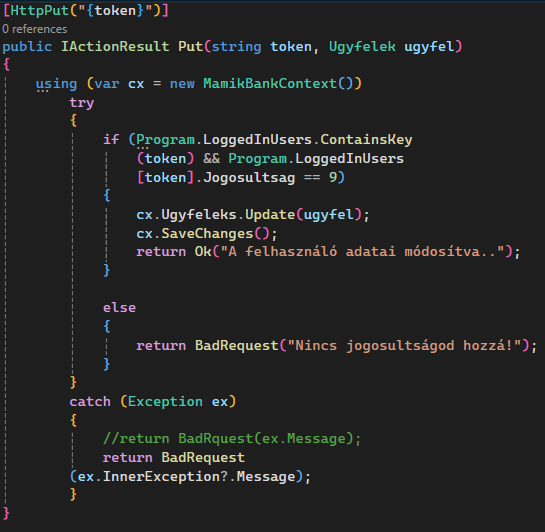
\includegraphics[width=8cm]{figures/ugyfelmodositas.png}
    \item \textbf{Ügyfél törlése}: Egy adott ügyfél eltávolítása az adatbázisból.
    \\
    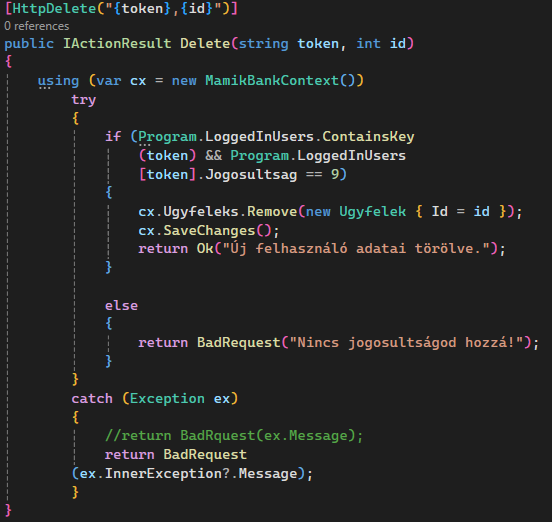
\includegraphics[width=8cm]{figures/ugyfeltorles.png}
\end{itemize}
\newpage
\section{Frontend bemutatása}
A MAMIK Bank frontend React.js és React Native alapokra épül, biztosítva a gyors, reszponzív és platformfüggetlen fejlesztést. A Virtual DOM technológia hatékony renderelést biztosít, míg TypeScript növeli a kódbiztonságot.  Az API-kommunikációt RESTful API és JWT alapú hitelesítés támogatja, garantálva a biztonságos adatkezelést.
\subsection{Weboldal áttekintése}
A weboldal főbb elemei:
\begin{itemize}
    \item \textbf{Főoldal}: Az ügyfelek üdvözlése és a szolgáltatások rövid bemutatása.
    \\
     
\includegraphics[width=8cm]{figures/Fooldal1.png}
    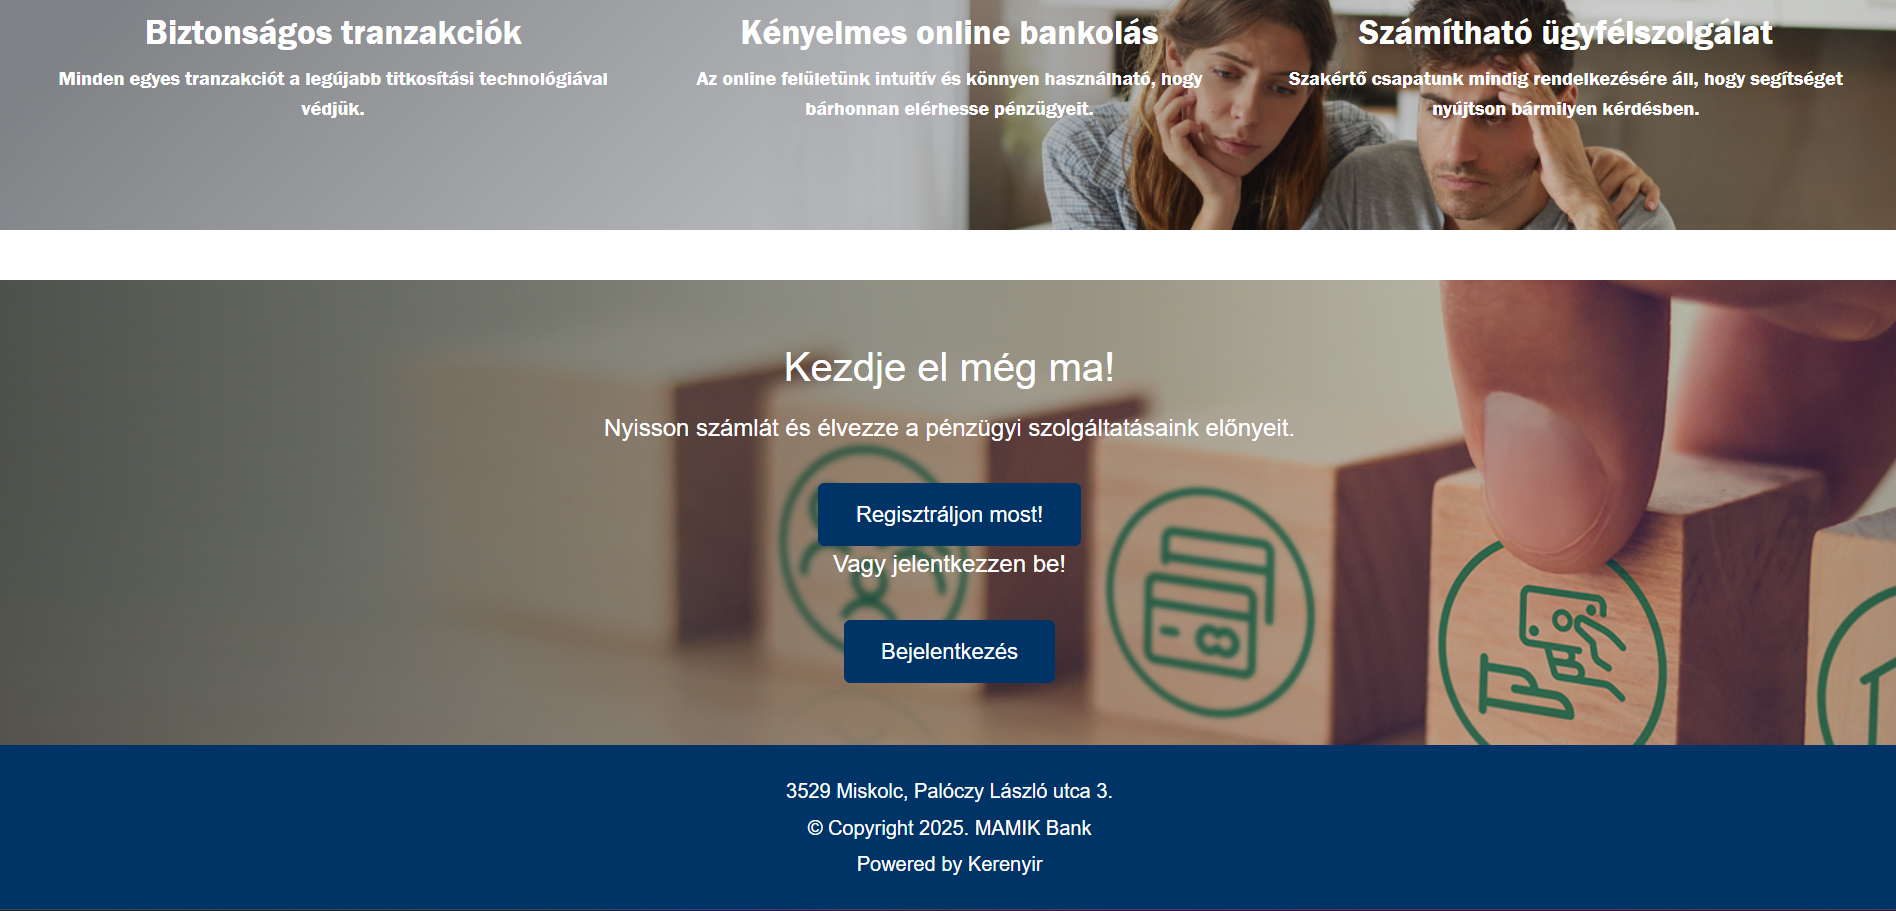
\includegraphics[width=8cm]{figures/Fooldal2.png}

    \item \textbf{Bejelentkezés/Kijelentkezés}: Az ügyfelek bejelentkezhetnek vagy kijelentkezhetnek fiókjukból.
    \\
    
\includegraphics[width=8cm]{figures/bejelfrontend.png}
    
\includegraphics[width=8cm]{figures/kijelfrontend.png}
    \item \textbf{Regisztráció}: Új ügyfelek számára lehetőség fiók létrehozására.
     \\
    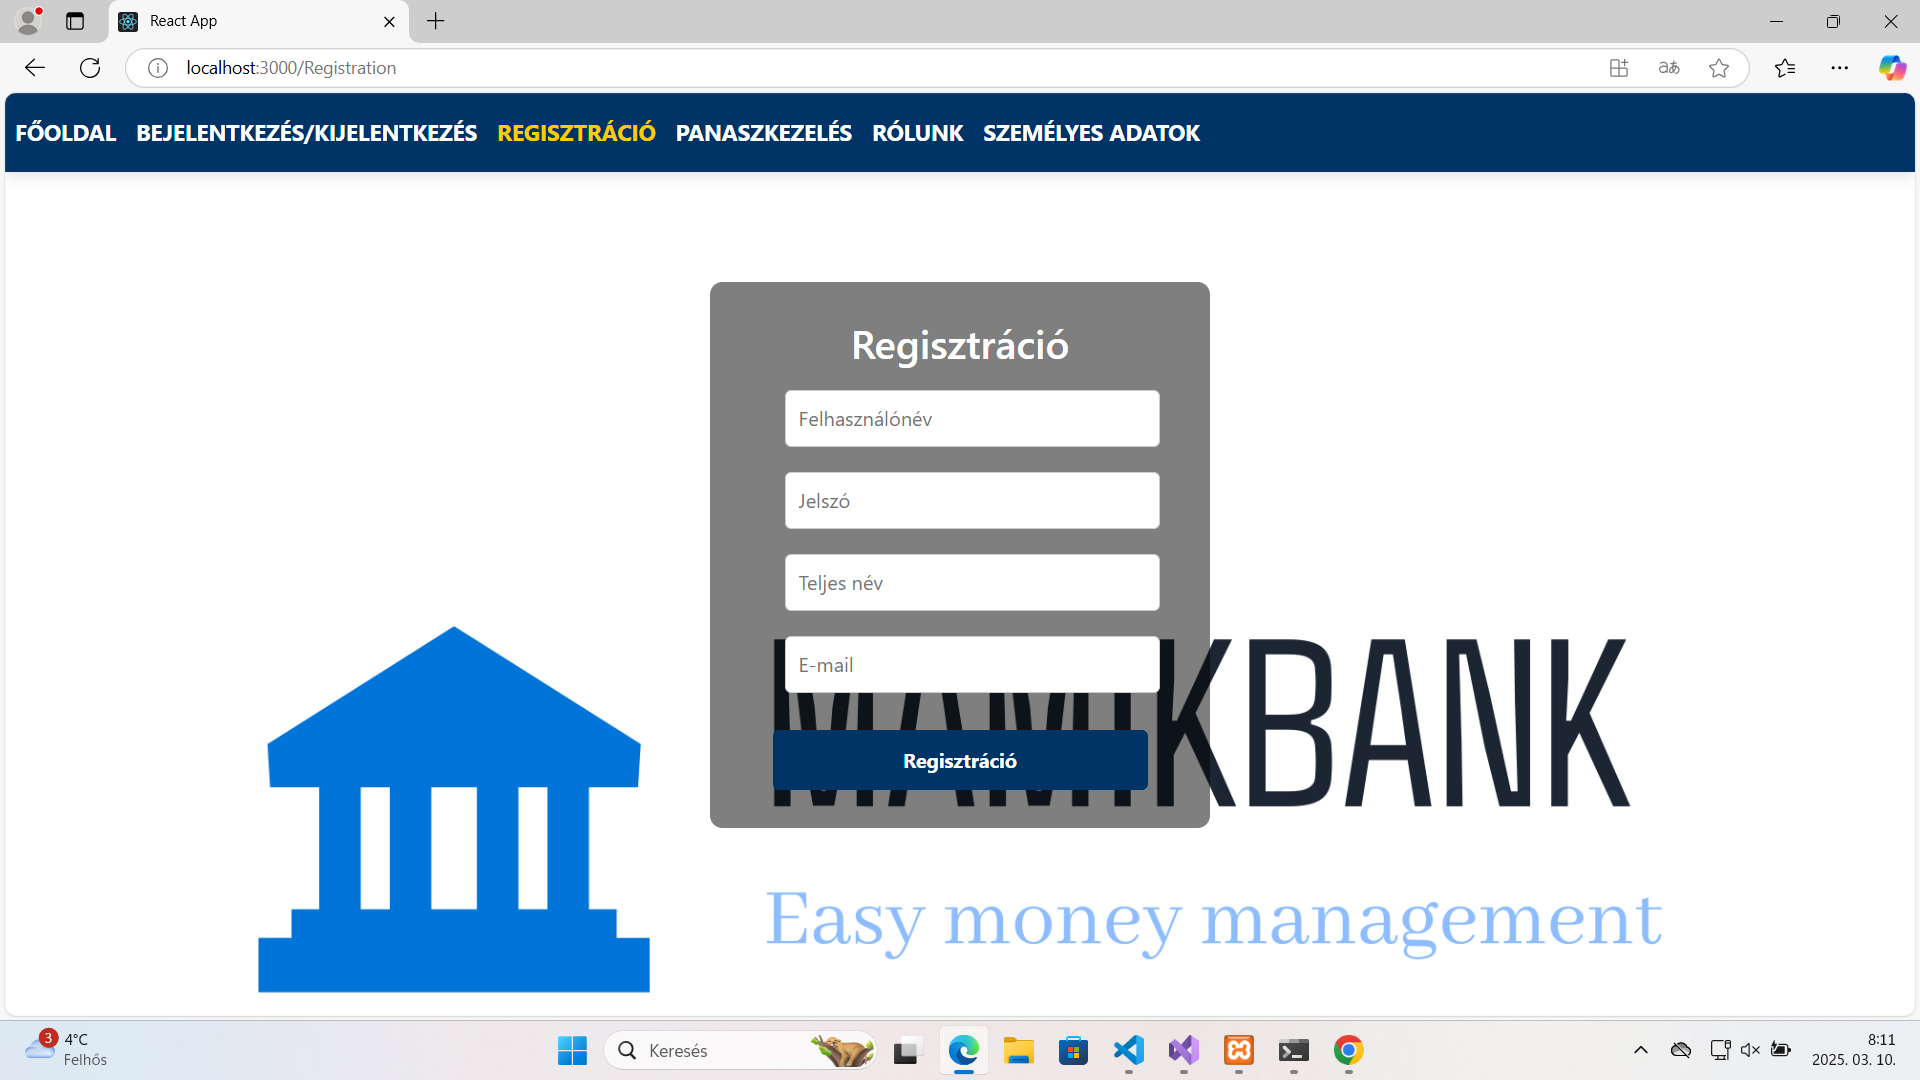
\includegraphics[width=10cm]{figures/regiszfrontend.png}
    \newpage
    \item \textbf{Panaszkezelés}: Ügyfelek panaszaikat és észrevételeiket kezelhetik.
    \\
    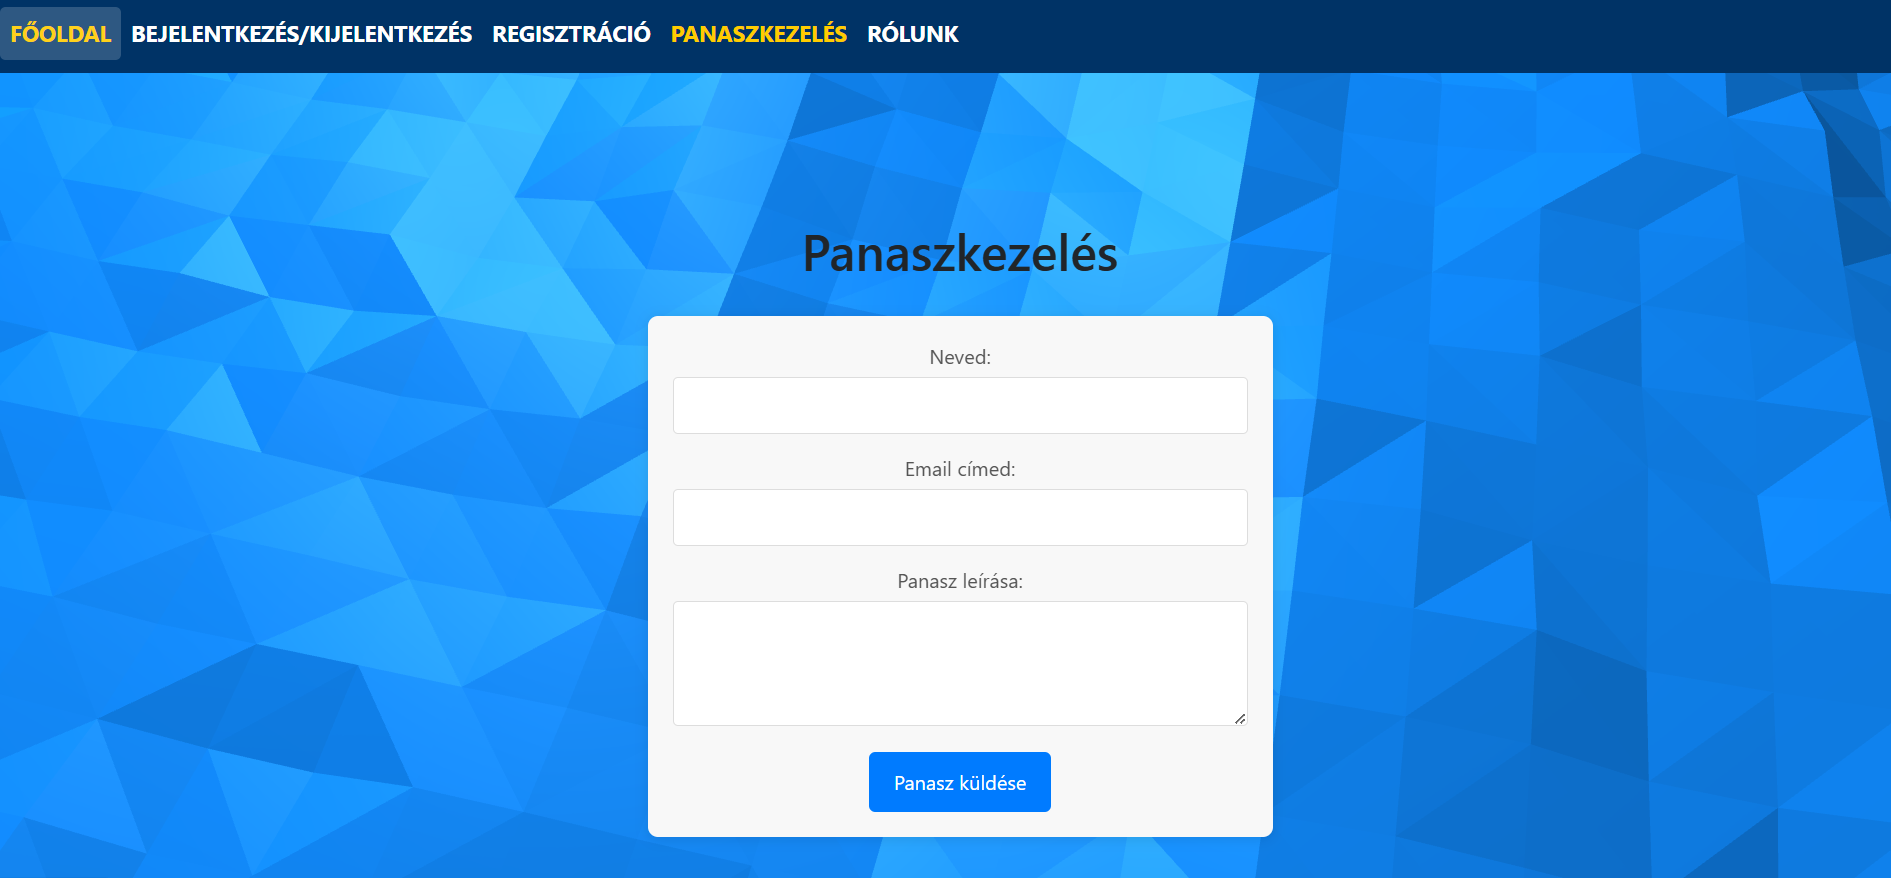
\includegraphics[width=10cm]{figures/panaszfrontend.png}
    
    \item \textbf{Rólunk}: Információ a bank történetéről és céljairól.
    \\
    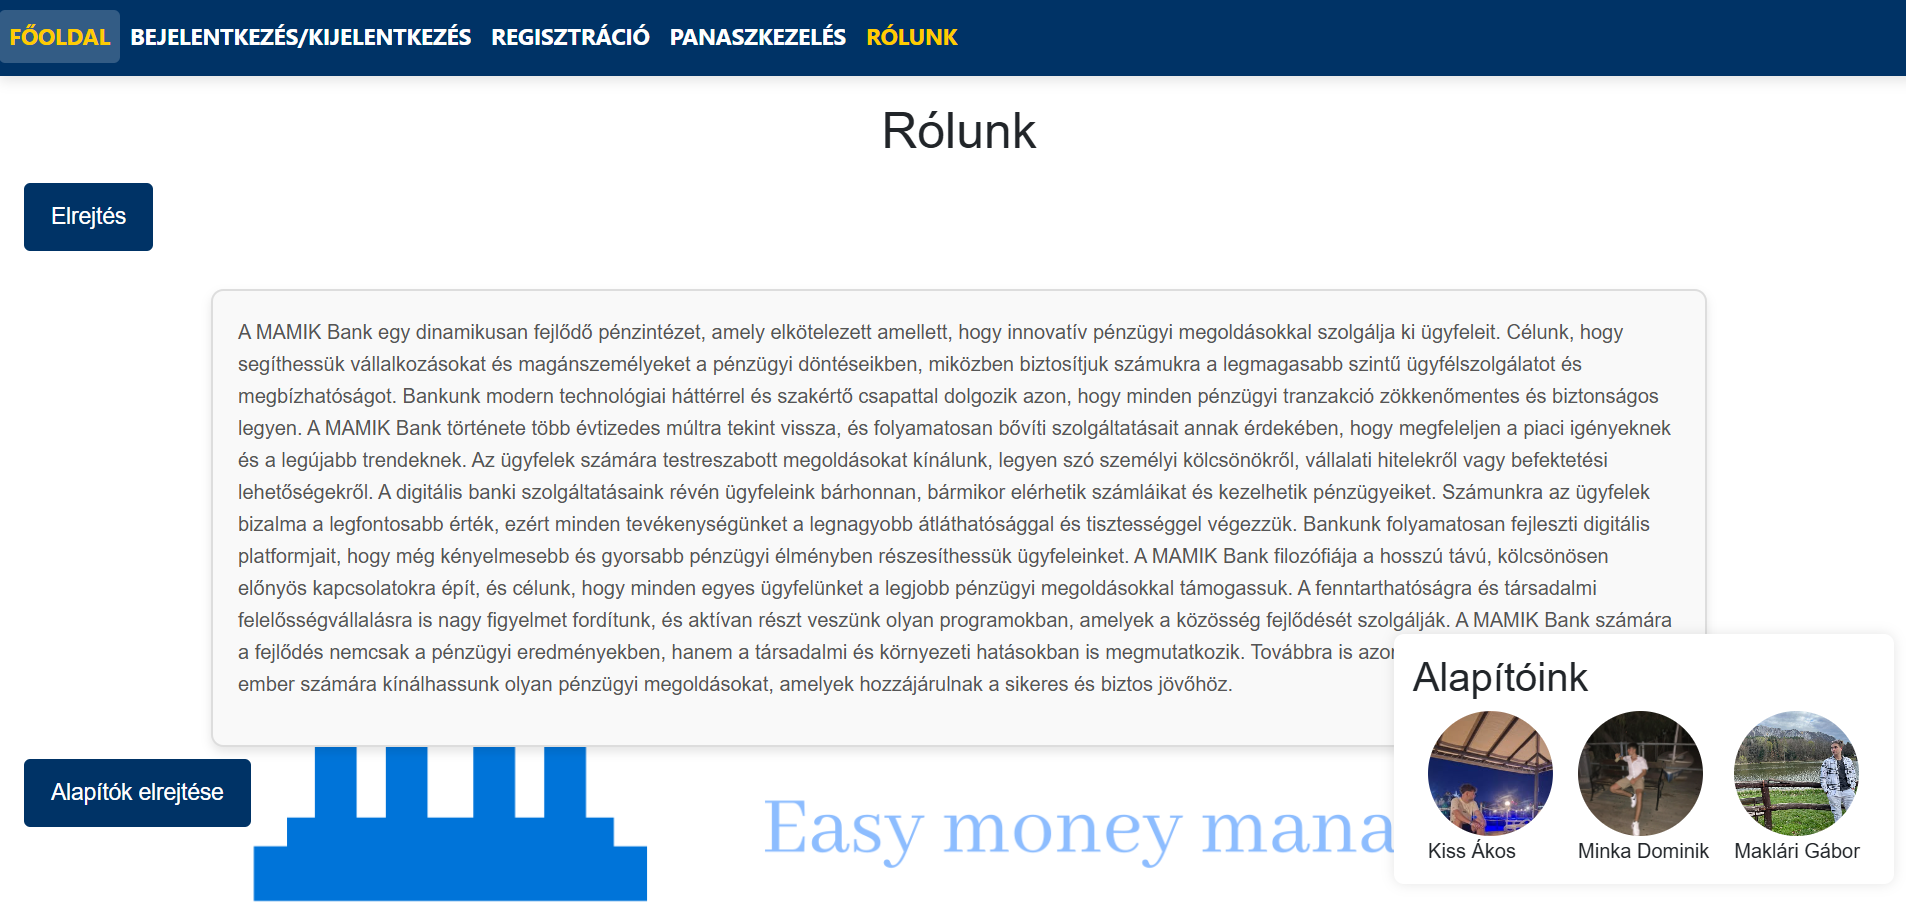
\includegraphics[width=12cm]{figures/rolunkfrontend.png}
    
\end{itemize}

\subsection{Megjelenés és design}
A weboldal modern, letisztult megjelenéssel rendelkezik:
\begin{itemize}
    \item A fejlécként szolgáló kék sávban találhatók a navigációs menüpontok.
    \item A főoldalon egy nagy üdvözlő szöveg és egy háttérkép látható.
    \item A bank logója egy kék színű ikon, amely egy oszlopos épületet ábrázol.
    \item A szlogen: \textit{``Easy money management''} (Egyszerű pénzkezelés).
\end{itemize}

\subsection{Funkciók}
A weboldal fő funkciói a következők:
\begin{itemize}
    \item Biztonságos bejelentkezés és kijelentkezés.
    \item Új ügyfelek számára regisztrációs lehetőség.
    \item Panaszkezelési rendszer az ügyfelek visszajelzéseinek feldolgozására.
    \item Banki szolgáltatások bemutatása és hozzáférhetővé tétele.
\end{itemize}
\newpage
\subsection{Banki személyes ügyek modális ablak}
\begin{itemize}
    \item Egyenlegünk tárolása megtakarításként is akár.
    \item Jelenlegi számla egyenleg(folyamatosan frissül egy-egy tranzakcióknál)
    \\ 
    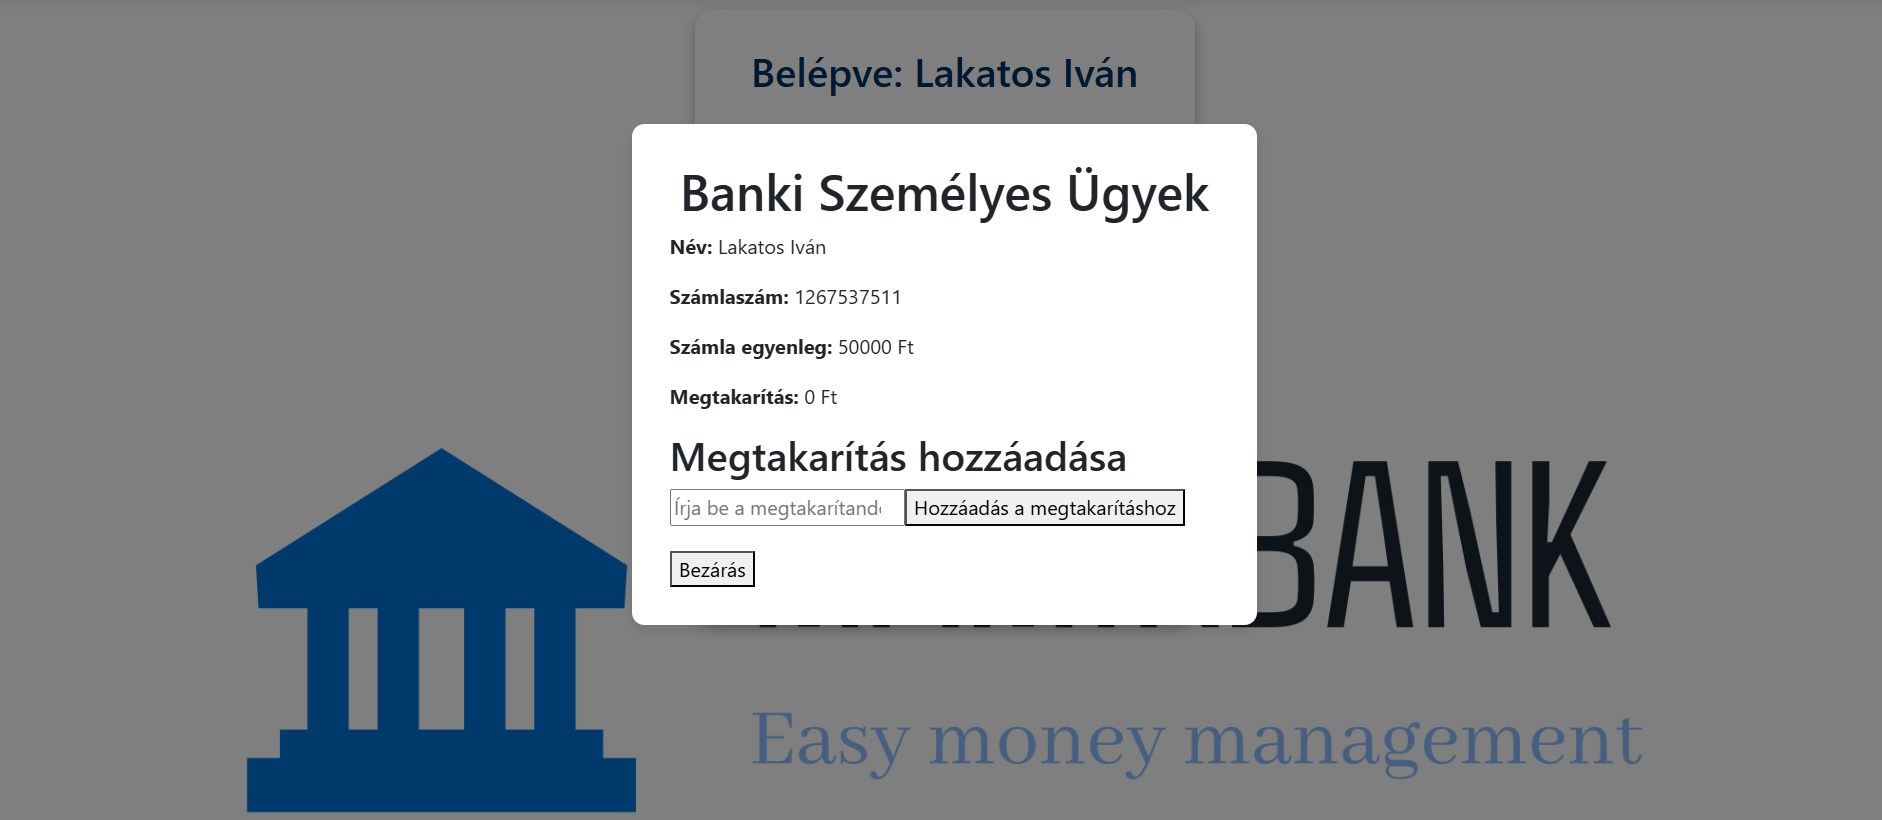
\includegraphics[width=10cm]{figures/szemelyesugyek.png}
\end{itemize}
    

\subsection{Biztonság és Ügyfélszolgálat}
A MAMIK Bank kiemelt figyelmet fordít a biztonságos bankolásra és az ügyfélszolgálati támogatásra:
\begin{itemize}
    \item \textbf{Biztonságos tranzakciók}: A legújabb titkosítási technológiákat alkalmazzuk minden egyes tranzakció védelmére.
    \item \textbf{Kényelmes online bankolás}: Intuitív és könnyen használható felületet biztosítunk, amely bárhonnan elérhető.
    \item \textbf{Számítható ügyfélszolgálat}: Szakértő csapatunk mindig rendelkezésére áll, hogy segítséget nyújtson bármilyen kérdésben. 
\end{itemize}
\newpage
\subsection{Funkciók és Jellemzők}
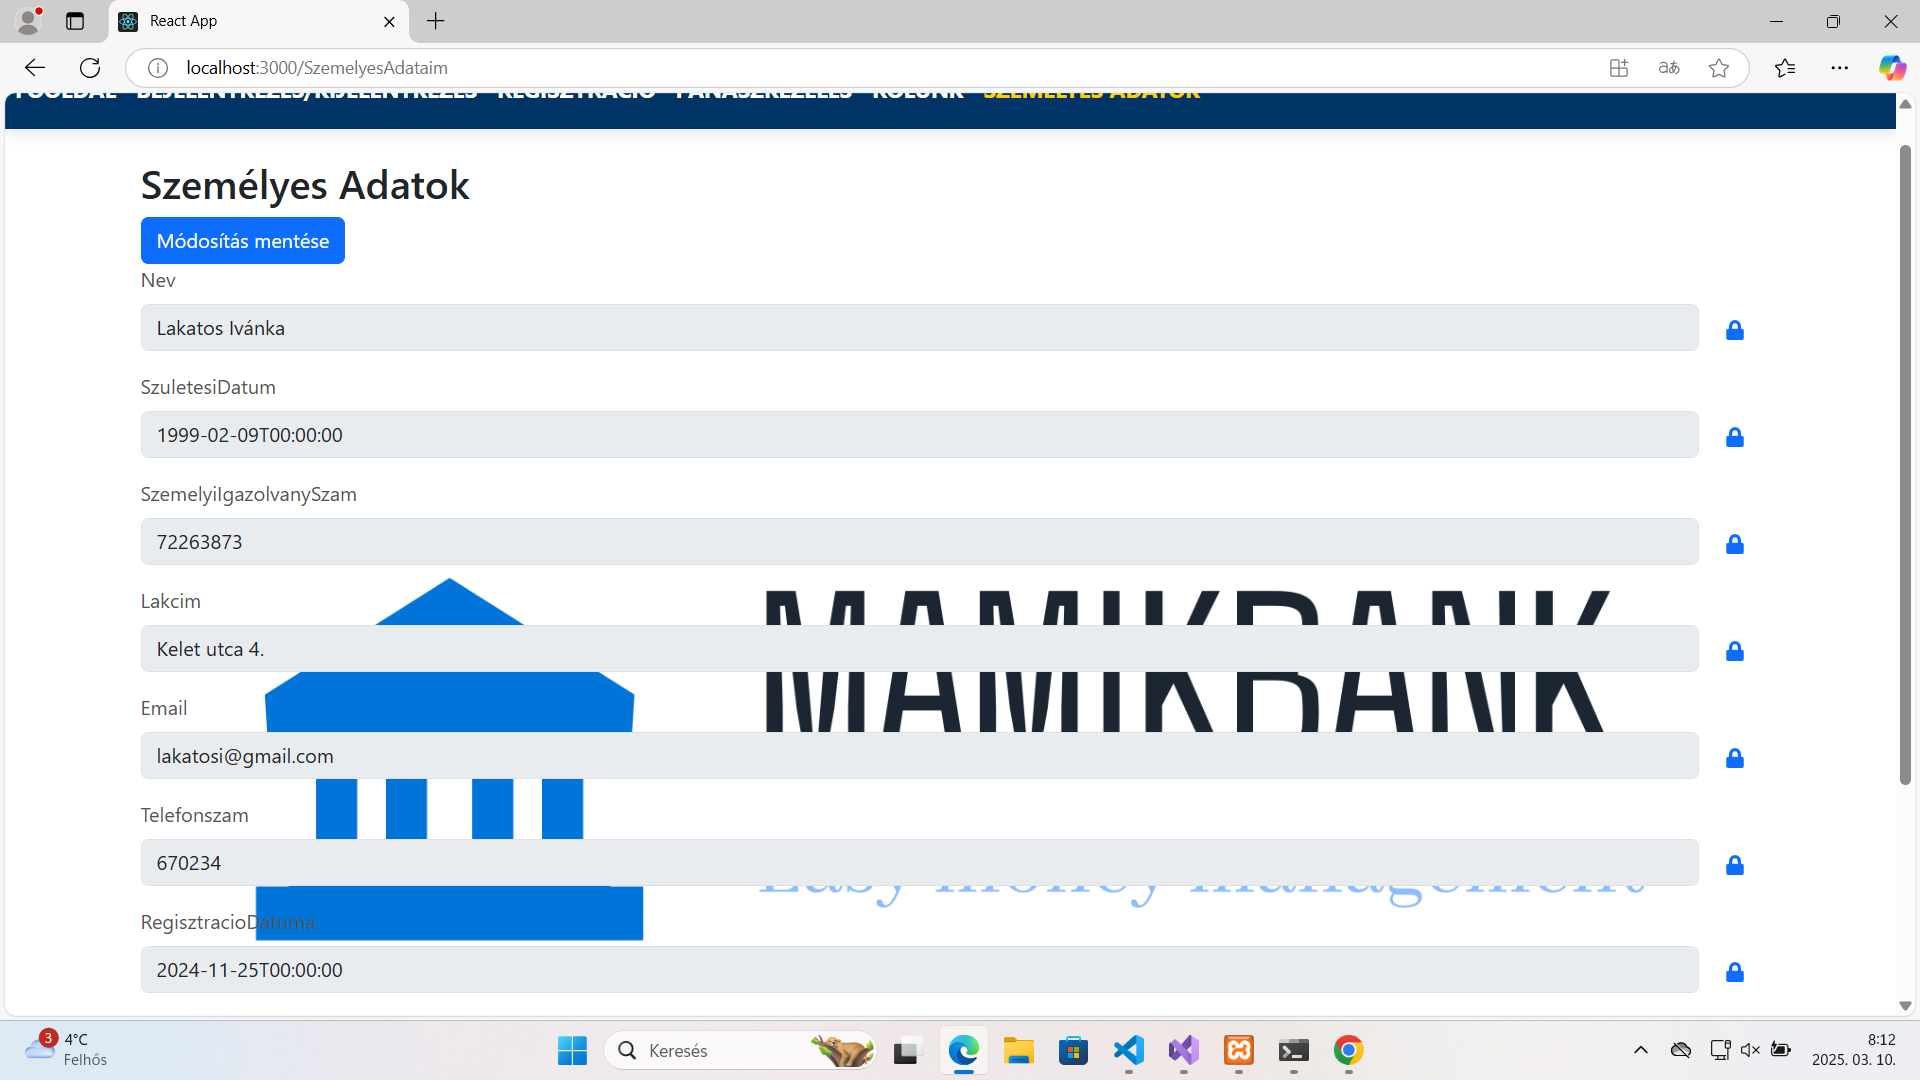
\includegraphics[width=12cm]{figures/szemadatfrontend.png}
\begin{itemize}
    \item \textbf{Személyes adatok megtekintése}: Az ügyfelek elérhetik és ellenőrizhetik alapvető személyes adataikat, mint például nevüket, születési dátumukat, lakcímüket és elérhetőségeiket.
    \item \textbf{Biztonságos hozzáférés}: A személyes adatok szerkesztése csak engedéllyel lehetséges. A zárolt mezők biztosítják, hogy érzékeny információk ne módosuljanak illetéktelenül.
    \item \textbf{Adatvédelmi intézkedések}: A rendszer titkosított adatkezelést alkalmaz, így a bizalmas ügyféladatok védve vannak az illetéktelen hozzáféréstől.
    \item \textbf{Egyszerű szerkesztés}: A „Módosítás mentése” gomb lehetővé teszi az ügyfelek számára az adatok frissítését, ha az adminisztrációs szabályok ezt engedélyezik.
    \item \textbf{Intuitív kezelőfelület}: A világos és könnyen olvasható űrlapok, valamint a jól strukturált adatelrendezés segítik az ügyfelek gyors eligazodását.
   
\end{itemize}


\subsection{Kapcsolat és Céginformációk}
A MAMIK Bank elérhetősége:
\begin{itemize}
    \item Cím: 3529 Miskolc, Palóczy László utca 3.
    \item Weboldal: https://mamikbank.hu
    \item Copyright 2025. MAMIK Bank
    \item Powered by Kerenyir
    \\
    
\includegraphics[width=10cm]{figures/Fooldal3.png}
\section{WPF bemutatása}
\end{itemize}



\end{itemize}
\newpage
\section{C\# .Net Web API}

\includegraphics[width=10cm]{figures/netapi.jpg}

\subsection{A Postman:}
\begin{itemize}
    \item API végpontok tesztelése: HTTP kérések küldése (GET, POST, PUT, DELETE stb.), válaszok megtekintése.
    Autentikációs módszerek támogatása: Alapértelmezett autentikáció (pl. Basic Auth, Bearer Token), OAuth 2.0 stb.
    Automatizált tesztelés: Automatizált tesztek írása és futtatása JavaScript segítségével.
    Kérés és válaszok dokumentálása: Az API végpontok és azok paramétereinek dokumentálása.
    
    \item A Postman nagyszerű eszköz a Web API-k fejlesztésében és tesztelésében. Segít a fejlesztőknek az API végpontok kipróbálásában, hibakeresésében, automatizált tesztek futtatásában és az API dokumentálásában. A fent bemutatott módon könnyen tesztelheted a C\# .NET Web API-kat a Postman segítségével, így gyorsan validálhat
    
\end{itemize}
\subsection{Unit tesztelés}
\begin{itemize}
    \item A Web API alkalmazások fejlesztésénél fontos a unit tesztelés. A .NET Core-ban használhatunk különböző tesztelési keretrendszereket:
    \item xUnit: Az egyik legnépszerűbb tesztelési keretrendszer a .NET alkalmazásokhoz.
    NUnit vagy MSTest: Más tesztelési keretrendszerek, amelyek szintén támogatják a .NET-tel való integrációt.
    Az unit teszteléshez gyakran használt eszközök:
    
    \item Moq: A mock-objektumok készítésére szolgáló könyvtár.
    FluentAssertions: Kifejező, olvasható állításokat (assertion) biztosít a tesztekhez.
\end{itemize}
\subsection{Hibakeresés (Debugging)}
\begin{itemize}
    \item A hibakeresés során a Visual Studio vagy Visual Studio Code lehetőséget ad a breakpointok elhelyezésére, az alkalmazás lépésenkénti futtatására és változók nyomon követésére.
\end{itemize}

\section{Swagger API Dokumentáció}

\begin{wrapfigure}{r}{0.4\textwidth} % 'r' a jobb oldalon jeleníti meg, 'l' balra helyezné
    \centering
    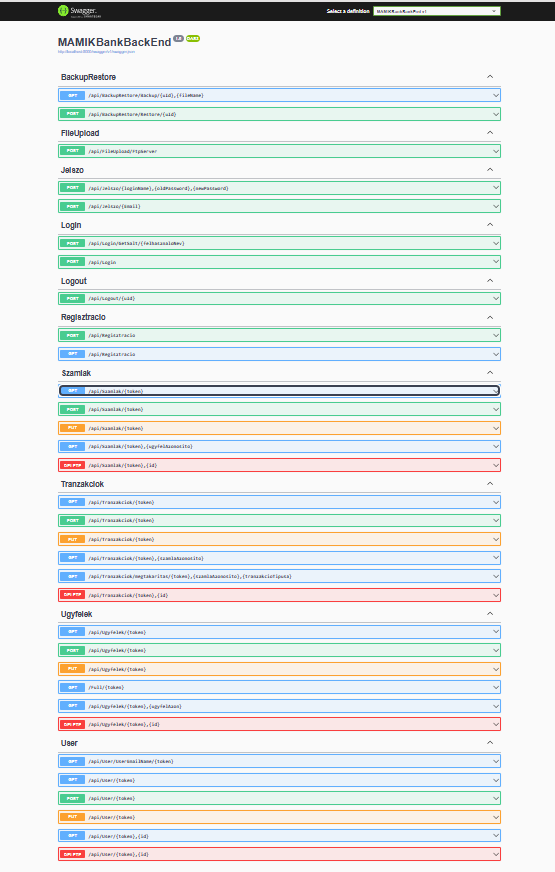
\includegraphics[width=0.48\textwidth]{figures/swagger.png} % A kép beillesztése
    
    \label{fig:example}
\end{wrapfigure}

Swagger (más néven OpenAPI) egy szabványos dokumentációs keretrendszer, amely lehetővé teszi a Web API automatikus dokumentálását és interaktív tesztelését. A Swashbuckle.AspNetCore csomag segítségével könnyen integrálhatjuk a Swagger-t a .NET Web API-ba.

Az alábbiakban bemutatjuk a MAMIK Bank backend API végpontjait és azok funkcióit:

\subsection{BackupRestore}
\begin{itemize}
    \item \textbf{Backup készítése}: Lehetővé teszi a banki adatok biztonsági mentését.
    \item \textbf{Backup visszaállítása}: A korábban elmentett adatok visszatöltése az adatbázisba.
\end{itemize}

\subsection{FileUpload}
\begin{itemize}
    \item \textbf{Fájlok feltöltése}: A rendszerbe történő fájl feltöltési lehetőség biztosítása.
\end{itemize}

\subsection{Jelző}
\begin{itemize}
    \item \textbf{Jelzők kezelése}: Figyelmeztetések és egyéb banki értesítések beállítása és frissítése.
\end{itemize}
\newpage
\section{Entity Framework}
\begin{figure}
    \centering
    
\includegraphics[width=10cm]{figures/entityframework.png}
\end{figure}
\subsection{Az ADO.NET Entitás-keretrendszer }
\begin{itemize}
   \item (EF, Entity Framework) egy objektum-relációs leképező keretrendszer a .NET keretrendszerhez.

   \item Az ADO.NET Entitás Keretrendszer architektúrája az alábbiakból áll össze növekvő absztrakciós sorrendben:

   \item  Adatforrás-specifikus kiszolgálók, amely absztrakciós ADO.NET felületeket használnak fel az adatbázis kapcsolathoz, amikor sémák szerint programozunk.

   \item Leképzés kiszolgáló, egy adatbázis függő kiszolgáló, amely lefordítja az Entitás SQL utasításfát lekérdezésekké az adatbázis natív SQL nyelvének megfelelően. Ez magába foglalja a tároló függő hidat, azt a komponenst, amely felelős a generikus utasításfák tárolófüggő utasításfákra való fordításáért.

   \item  EDM elemző és nézet leképezés, amely felhasználja az adatmodell SDL specifikációját, és az alapján, ahogyan az leképez a relációs modellre, lehetővé teszi az elméleti modellben történő programozást. A relációs sémából létrehoz nézeteket, amely megfelel az elméleti modellnek. Összegyűjti az információkat különböző táblákból entitásokat kialakítva belőlük, és szétosztja, illetve frissíti az entitás adatait a különböző táblákban, függetlenül attól, mely táblák tartoznak az entitáshoz.

   \item Lekérdezés és frissítés csővezeték, azaz pipeline, folyamat-lekérdezések, filterek és frissítési kérelmek küldése, hogy átalakítsa őket kanonikus utasításfákká, amelyeket tároló specifikus lekérdezésekké alakít a leképzés szolgáltató segítségével.
   \item   Metaadat szolgáltatók, ez kezeli az összes entitáshoz rendelt metaadatot, kapcsolatokat és leképezéseket.
   \item  Tranzakciók, elérhetővé teszik a tár tranzakciós szolgáltatásait. Amennyiben a felhasznált tároló nem támogatja a tranzakciókat, a szükségeknek megfelelően ez a réteg valósítja meg ezeket.

   \item   Koncepciós réteg API, egy olyan környezet, amely lehetővé teszi a koncepciós séma programozását. Követi az ADO.NET mintákat Connection objektumok használatával, hogy leképezés szolgáltatókra hivatkozzon, használja a Command objektumokat hogy leképezések küldjön el, és EntityResultSets vagy EntitySets-ként adja vissza a végeredményt.

   \item Kapcsolat nélküli/leválasztott komponensek, helyileg tárolják az adathalmazt és az entitás halmazokat, hogy kihasználják az ADO.NET Entitás Keretrendszer lehetőségeit egy alkalmanként csatlakozó környezetben.
   \item Beágyazott adatbázis: az ADO.NET Entitás Keretrendszer magában foglal egy könnyű súlyú adatbázist a relációs adatok felhasználó oldali gyorsítótárazására.

    \item   Tervező eszközök, a Leképezés Tervezőhöz hasonlóan ezek szintén beépítettek az ADO.NET Entitás Keretrendszerbe. Egyszerűsíti a leképezéseken végzett feladatokat egy koncepciós sémából relációs sémába és meghatározza, hogy az entitás típus adott tulajdonságai mely táblához tartoznak az adatbázisban.
    \item Programozási réteg, rajta keresztül férünk hozzá az EDM-hez mint programozási konstrukcióhoz, amely felhasználható a programozási nyelveken.

     \item  Objektum szolgáltatások, automatikusan generálják a kódot CLR osztályokhoz, amelyek az entitásnak megfelelő tulajdonságokkal rendelkeznek, ezzel lehetővé téve az entitások .NET objektumokként való példányosítását.

     \item   Web szolgáltatások, az entitások segítségükkel web szolgáltatásként elérhetőek.
     \item Magas szintű szolgáltatások, mint például a jelentés szolgáltató, amely entitásokkal dolgozik relációs adatok helyett.
    
    \end{itemize}
    \subsection{CRUD:}
    \begin{itemize}
        \item CRUD a Create (Létrehozás), Read (Olvasás), Update (Módosítás) és Delete (Törlés) rövidítése. Ezek a négy alapvető művelet végezhetők el adatokkal adatbázisban vagy bármely más tartós tárolóban. A CRUD műveletek elengedhetetlenek az alkalmazásokban található adatok kezeléséhez és manipulálásához.
     
    \end{itemize}

\chapter*{Összegzés}
\addcontentsline{toc}{chapter}{Összegzés}
A banki alkalmazásunk egy modern és biztonságos pénzügyi platform, amely különféle technológiák és szolgáltatások integrációjával biztosítja a felhasználók számára a gördülékeny és hatékony banki ügyintézést.
\newline\newline
\textbf{Adatbáziskezelés}

A rendszerünk MySQL és MariaDB adatbázisokat használ, amelyek biztosítják az adatok gyors és megbízható tárolását. Az adminisztrációs feladatokhoz a PHPMyAdmin felületet alkalmazzuk.
\newline\newline
\textbf{Frontend és Backend Technológiák}
A frontend fejlesztéséhez React Native technológiát alkalmazunk, amely platformfüggetlen mobilalkalmazásokat tesz lehetővé. A backend oldalon a .NET Web API keretrendszert használjuk, biztosítva a stabil és biztonságos adatkezelést. A Postman tesztelési eszközzel ellenőrizzük az API működését.
\newline\newline
\textbf{Swagger API Dokumentáció}

A rendszerünk Swagger API dokumentációval rendelkezik, amely részletes információkat nyújt a végpontok működéséről, beleértve a biztonsági mentéseket, fájlok feltöltését, regisztrációt, számlák és tranzakciók kezelését, valamint az ügyfelek adatait.
\newline\newline
\textbf{Megjelenés és Funkcionalitás}

A weboldalunk modern és letisztult dizájnnal rendelkezik, amely könnyen navigálható és biztosítja az összes szükséges banki funkciót. A felhasználói élmény és a biztonság kiemelt szerepet kap, a személyes adatok védelme érdekében.
\newline\newline

\newpage
\Huge\begin{center}
	\textbf{Köszönetnyilvánítás}	
\end{center}\normalsize
Ezúton szeretnénk kifejezni hálánkat és köszönetünket mindazoknak, akik hozzájárultak a vizsgaremekünk elkészítéséhez és sikeres megvalósításához.
\newline
\newline
Különösen szeretnénk megköszönni Deák Csabának, Kerényi Róbertnek és Németh Bencének az értékes segítséget, szakmai tanácsokat és a projekt során tanúsított támogatást. Nélkülük nem sikerült volna ilyen szintű eredményt elérni a banki alkalmazás program megvalósításában.
\newline
Köszönjük az együttműködést, az ötleteket, és minden egyes pillanatot, amelyet a közös munka során együtt tölthettünk!
\begin{figure}[h]
    \centering
    
\includegraphics[width=\textwidth]{figures/mamikbank-high-resolution-logo.png}

\end{figure}

\begin{thebibliography}{2}
\addcontentsline{toc}{chapter}{\bibname}
\bibitem{internet} \textsc{PHPMyAdmin}: \emph{Az információkat a wikipédiáról szereztük az adatbázis alapjairól}, 2024.10.22-én, \url{https://en.wikipedia.org/wiki/PhpMyAdmin}
\bibitem{internet} \textsc{React Native}: \emph{Az információkat a React oldaláról és a wikipédiáról gyűjtöttük össze a react alapjairól }, 2024.11.5-én, \url{https://hu.legacy.reactjs.org/tutorial/tutorial.html}
\bibitem{internet} \textsc{.NET Web API}: \emph{Az információkat a Loadfocus oldaláról  gyűjtöttük össze a .NET Web API alapjairól }, 2024.11.18-án, \url{https://loadfocus.com/hu-hu/glossary/crud-operations-what-is-crud}
\bibitem{internet} \textsc{ENTITY FRAMEWORK}: \emph{Az információkat a Wikipédia oldaláról  gyűjtöttük össze a Entity Framework alapjairól }, 2024.11.21-én, \url{https://en.wikipedia.org/wiki/Entity_Framework}
\bibitem{internet} \textsc{JWT}: \emph{Az információkat a JWT oldaláról  gyűjtöttük össze a JWT(Json Web Token) alapjairól }, 2024.11.21-én, \url{https://jwt.io/}
\end{thebibliography}
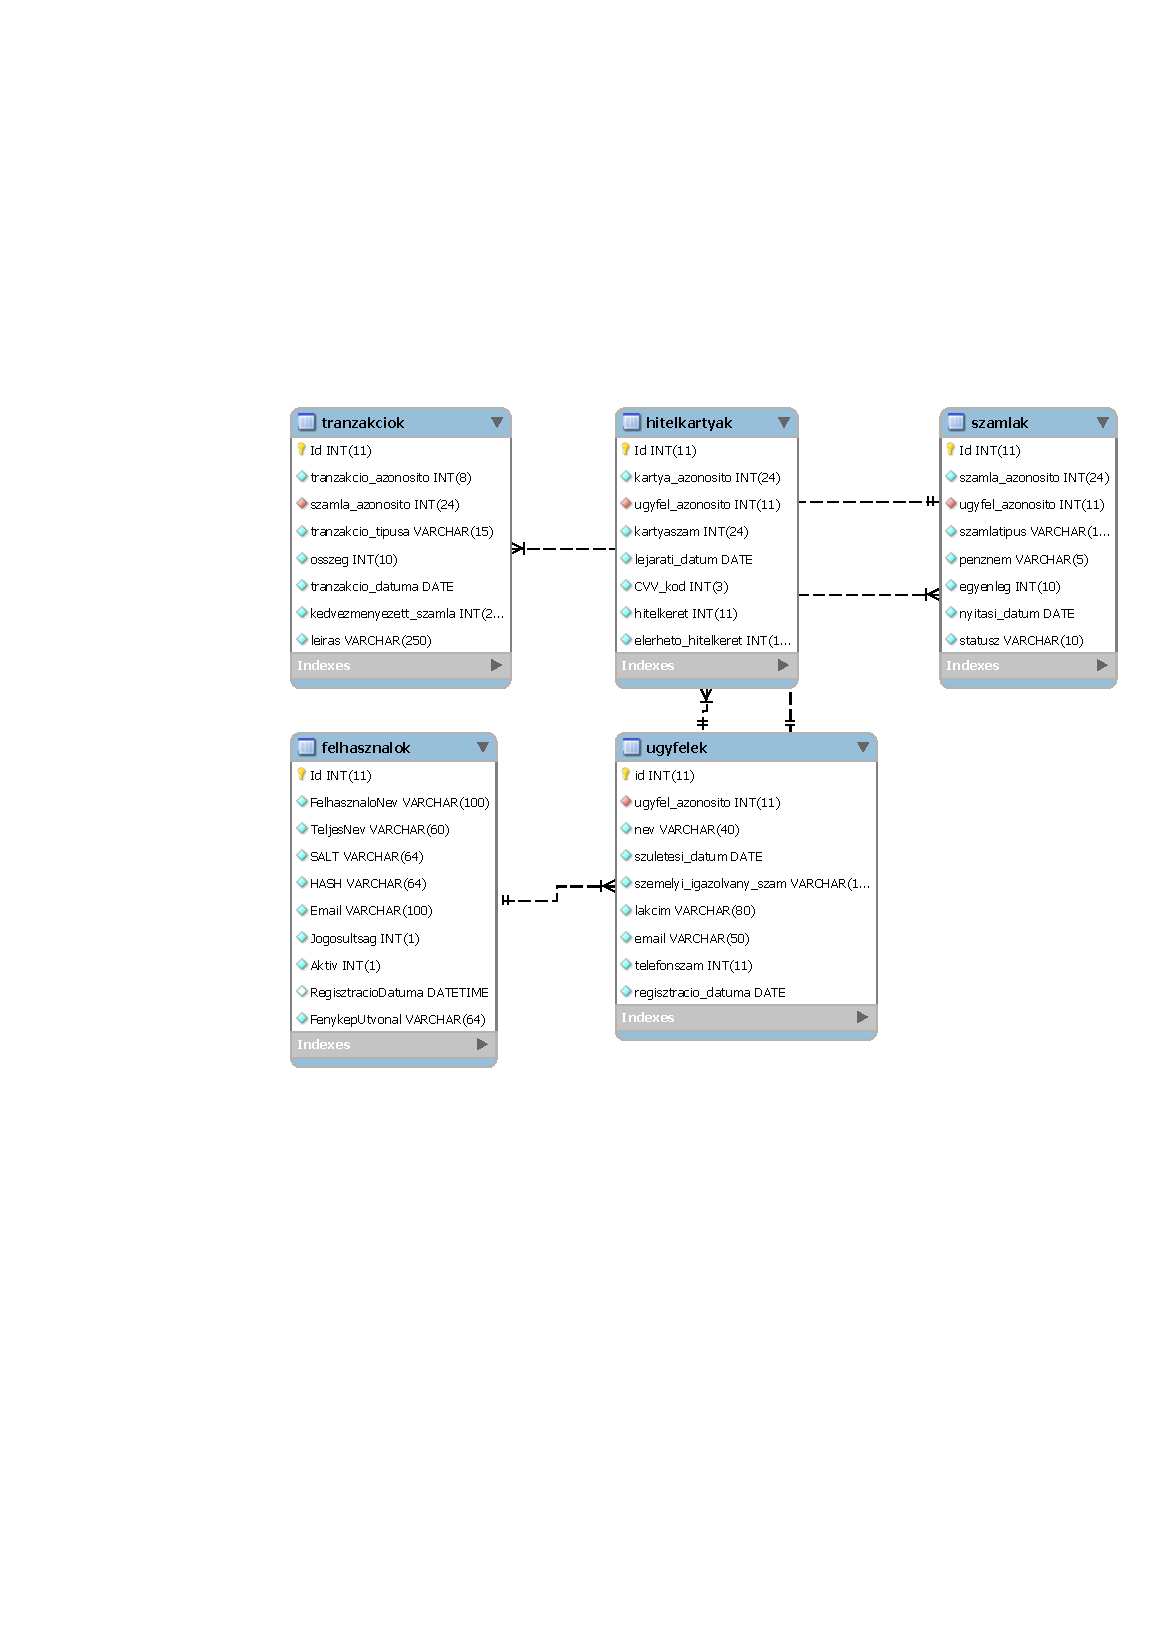
\includepdf{figures/adatb.pdf}
% Ide lehet szkennelt dokumentumot, dokumentumokat beszúrni
%\includepdf{}

\end{document}